% 01 --- Introduction: Simulation / Modeling / Computational Experiments / Representation / Objectives / Applications
\section{Introduction to Molecular Simulation}

\subsection{What is Simulation?}
\begin{frame}{What is Simulation? --- Control Over Numbers on a Chip}
	\hfuzz=15pt
	\begin{columns}[T,onlytextwidth]
		\column{0.58\textwidth}
		\begin{pitemize}
			\item \neoncyan{Simulation} = computable mirror of reality
			\item \textbf{Control} \ensuremath{\rightarrow} numbers you \glow{ingrain} in silicon
			\item Chip = deterministic universe you design
			\item Input: \inlinecode{numbers} \ensuremath{\rightarrow} Output: \inlinecode{properties}
			\item \textbf{Why?} --- experiment impossible / dangerous / expensive
		\end{pitemize}
		\vspace{2mm}
		\begin{infobox}[Chip = Lab]
			\footnotesize Transistors \ensuremath{\rightarrow} arithmetic \ensuremath{\rightarrow} models \ensuremath{\rightarrow} atoms \ensuremath{\rightarrow} materials \ensuremath{\rightarrow} life
		\end{infobox}
		\column{0.45\textwidth}
		\begin{center}
			\begin{tikzpicture}[scale=0.92, every node/.style={font=\small}]
				% Chip with pins
				\node[draw=accentcyan,rounded corners=2mm,fill=darkgray,minimum width=3.2cm,minimum height=1.4cm,align=center,drop shadow={shadow xshift=0.5mm,shadow yshift=-0.5mm,opacity=0.5}] (chip) at (0,2.6) {\color{fgwhite}\bfseries\normalsize CPU/GPU\\\color{softgray}\footnotesize\ttfamily chip};
				% Chip pins — short stubs above and below the box only
				\foreach \x in {-1.0,-0.5,0,0.5,1.0} {\draw[accentcyan,thick] (\x,3.3) -- (\x,3.55); \draw[accentcyan,thick] (\x,1.9) -- (\x,1.65);}
				% Simulation
				\node[draw=neongreen,rounded corners=2mm,fill=bgdark,minimum width=3.5cm,minimum height=1.3cm,align=center,drop shadow] (sim) at (0,0.3) {\color{neongreen}\bfseries\normalsize Simulation\\\color{fgwhite}\footnotesize $F=ma$\,,\,$U(\mathbf{r})$};
				% Observables
				\node[draw=neonyellow,rounded corners=2mm,fill=bgdark,minimum width=3.5cm,minimum height=1.2cm,align=center,drop shadow] (obs) at (0,-2.0) {\color{neonyellow}\bfseries\normalsize Observables\\\color{fgwhite}\footnotesize $P,\ \rho,\ D,\ \Delta G$};
				% Arrows with labels
				\draw[-{Stealth[length=4mm,width=3mm]},thick,accentcyan] (chip.south) -- (sim.north) node[midway,right=8pt,font=\footnotesize,color=accentcyan]{model};
				\draw[-{Stealth[length=4mm,width=3mm]},thick,neongreen] (sim.south) -- (obs.north) node[midway,right=8pt,font=\footnotesize,color=neongreen]{measure};
				\only<2>{\node[draw=neonpink,fill=neonpink!12,rounded corners=2mm,inner sep=2.5mm,align=center] at (0,4.0) {\color{neonpink}\bfseries\small you control $\Delta t,\,T,\,P$!\\\color{bgblack}\footnotesize\ttfamily dt, thermostat, barostat};}
				\only<3>{\node[draw=accentcyan,fill=accentcyan!10,rounded corners=1mm,inner sep=2mm,align=center] at (3.2,0.3) {\color{accentcyan}\footnotesize\bfseries $10^9$ steps $\to$ $1\,\mu$s};}
			\end{tikzpicture}
		\end{center}
	\end{columns}
\end{frame}

\begin{frame}{Interpretation --- Simulation}
	\interpret{
		\textbf{Simulation} · mimic reality in code · \textbf{control} numbers \ensuremath{\rightarrow} control physics · \textbf{chip} = lab · \textbf{reproducible} · \textbf{cheap} \textit{what-if} · \textbf{not} magic --- model quality = result quality
	}
\end{frame}

\subsection{Molecular Modeling \& Orbital Concepts}
\begin{frame}{Molecular Modeling --- From Orbitals to Atoms}
	\begin{columns}[T,onlytextwidth]
		\column{0.55\textwidth}
		\begin{pitemize}
			\item \neoncyan{Orbitals} $\psi_{n\ell m}$ \ensuremath{\rightarrow} electron density
			\item Hydrogenic: $ \hat H\psi = E\psi $, $\psi_{100}\propto e^{-r/a_0}$
			\item Atoms \ensuremath{\rightarrow} \textbf{bonds}, \textbf{angles}, \textbf{dihedrals}
			\item Models: \textbf{Quantum} (DFT) vs \textbf{Classical} (balls+springs)
			\item Precision ladder: \glowstrong{hydrogenic} \ensuremath{\rightarrow} DFT \ensuremath{\rightarrow} force field
		\end{pitemize}
		\column{0.45\textwidth}
		\begin{tikzpicture}[scale=1.0]
			\shade[ball color=neonblue!70] (0,0) circle (0.35cm); \node[color=white] at (0,0){H};
			\shade[ball color=neongreen!70] (1.2,0.6) circle (0.28cm); \node[color=white] at (1.2,0.6){H};
			\shade[ball color=neonpink!70] (1.2,-0.6) circle (0.32cm); \node[color=white] at (1.2,-0.6){O};
			\draw[thick,accentcyan] (0,0) -- (1.2,0.6); \draw[thick,accentcyan] (0,0) -- (1.2,-0.6);
			\draw[dashed,neonyellow] (1.2,0.6) arc (60:-60:0.7cm);
			\node[color=neonyellow] at (1.8,0) {$\theta$};
			\only<2>{\draw[accentcyan,thick,dashed] (0.4,0.9) -- (0.4,1.6) node[above,color=accentcyan]{orbital cloud};}
		\end{tikzpicture}
		\vspace{2mm}
		{\footnotesize\color{softgray} Wireframe $\leftrightarrow$ Ball-and-stick $\leftrightarrow$ Space-filling}
	\end{columns}
\end{frame}

\begin{frame}{Interpretation --- Modeling}
	\interpret{
		\textbf{Modeling} · choose resolution · \textbf{orbitals} = quantum truth · \textbf{atoms} = classical shortcut · \textbf{precision} costs · \textbf{ball-and-stick} = human eye model
	}
\end{frame}

\subsection{Computational Experiments}
\begin{frame}{Computational Experiments --- The Third Pillar}
	\begin{columns}[T,onlytextwidth]
		\column{0.5\textwidth}
		\venn{Theory}{Experiment}{Simulation}
		\column{0.5\textwidth}
		\begin{pitemize}
			\item \textbf{Theory} \ensuremath{\rightarrow} equations
			\item \textbf{Experiment} \ensuremath{\rightarrow} nature answers
			\item \textbf{Simulation} \ensuremath{\rightarrow} \glow{nature under your conditions}
			\item Controlled $T,P,N$, perfect observation
			\item Falsifiable, reproducible
		\end{pitemize}
	\end{columns}
	\vspace{3mm}
	\begin{alertbox}[Not a video game]
		\footnotesize You don't watch molecules --- you \textbf{measure} them: $g(r)$, MSD, $\Delta G$.
	\end{alertbox}
\end{frame}

\subsection{Molecular Representation}
\begin{frame}{Molecular Representation --- How Computers See Molecules}
	\begin{columns}[T,onlytextwidth]
		\column{0.5\textwidth}
		\begin{pitemize}
			\item \textbf{Ball-and-stick}: atoms=spheres, bonds=sticks
			\item \textbf{Wireframe}: bonds only --- topology
			\item \textbf{Space-filling}: vdW radii --- volume
			\item \textbf{Cartoon}: proteins \ensuremath{\rightarrow} helices/sheets
			\item All derived from \inlinecode{coordinates + bonds}
		\end{pitemize}
		\column{0.5\textwidth}
		\memeinclude[width=0.9\linewidth]{assets/memes/water_meme.png}
		{\footnotesize\color{softgray} Meshy \texttt{nano-banana} --- water waving}
	\end{columns}
\end{frame}

\begin{frame}{Representation Zoo}
	\begin{columns}[T,onlytextwidth]
		\column{0.24\textwidth}
		\begin{center}
			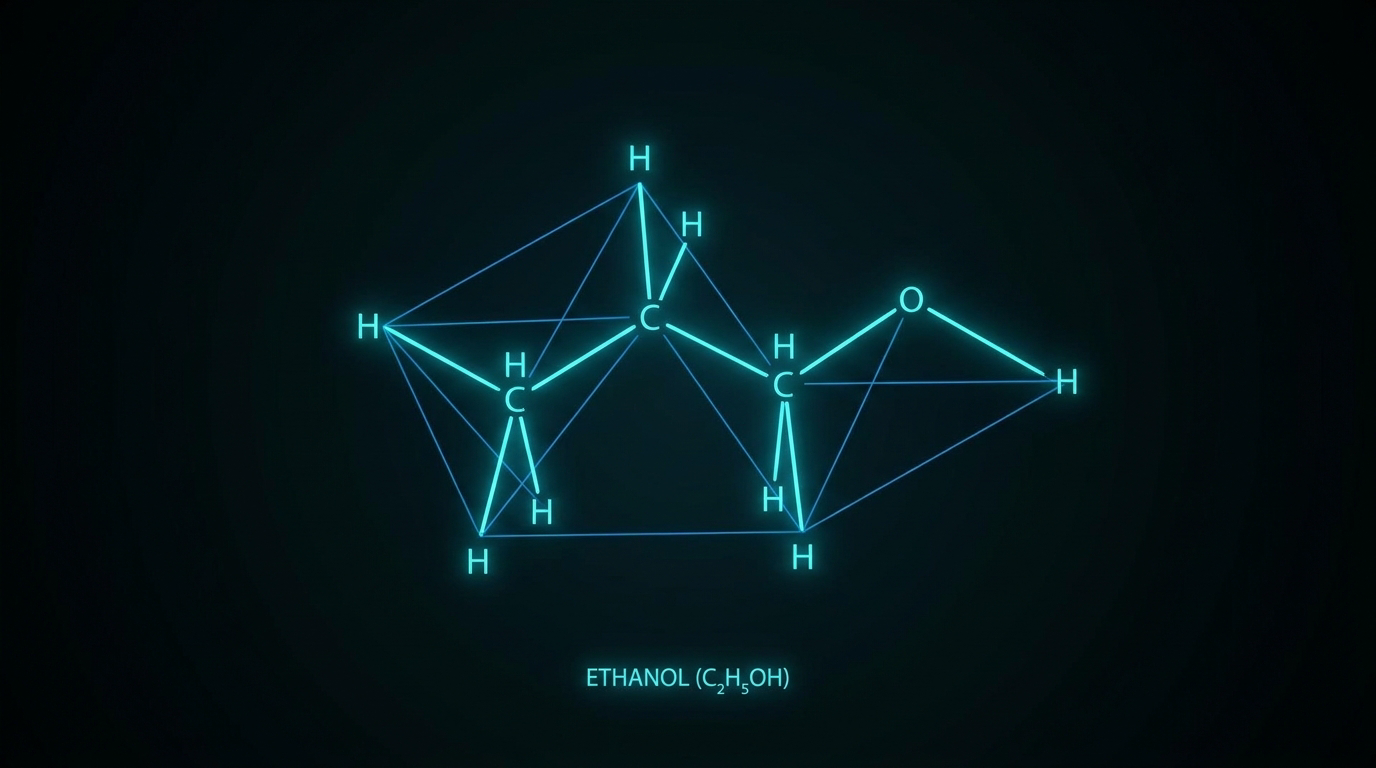
\includegraphics[width=\linewidth]{assets/figures/wireframe.png}
			{\footnotesize\color{softgray} Wireframe}
		\end{center}
		\column{0.24\textwidth}
		\begin{center}
			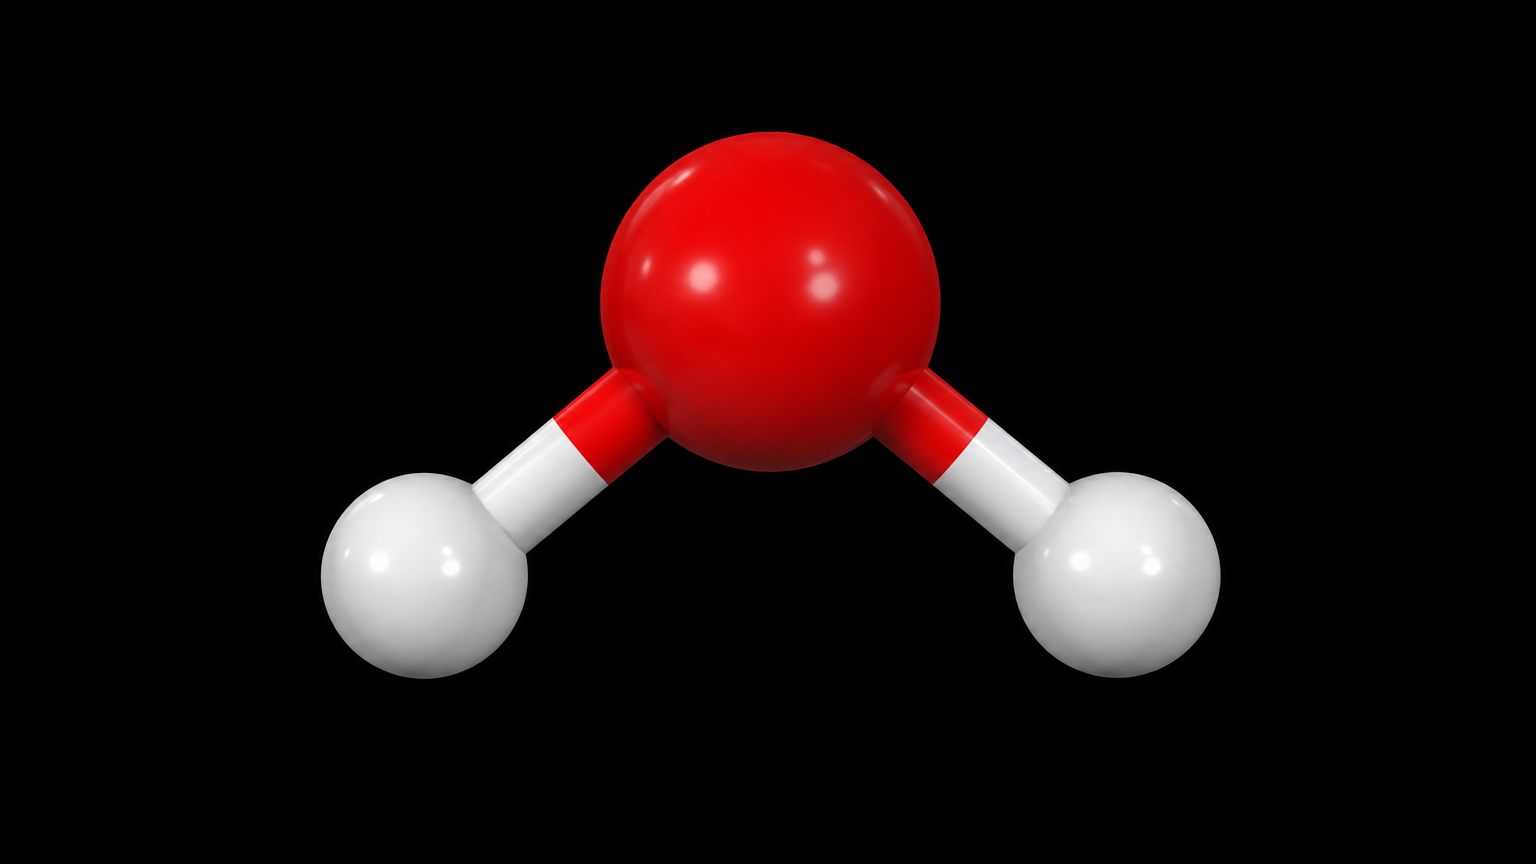
\includegraphics[width=\linewidth]{assets/figures/ball_stick_water.png}
			{\footnotesize\color{softgray} Ball-and-stick}
		\end{center}
		\column{0.24\textwidth}
		\begin{center}
			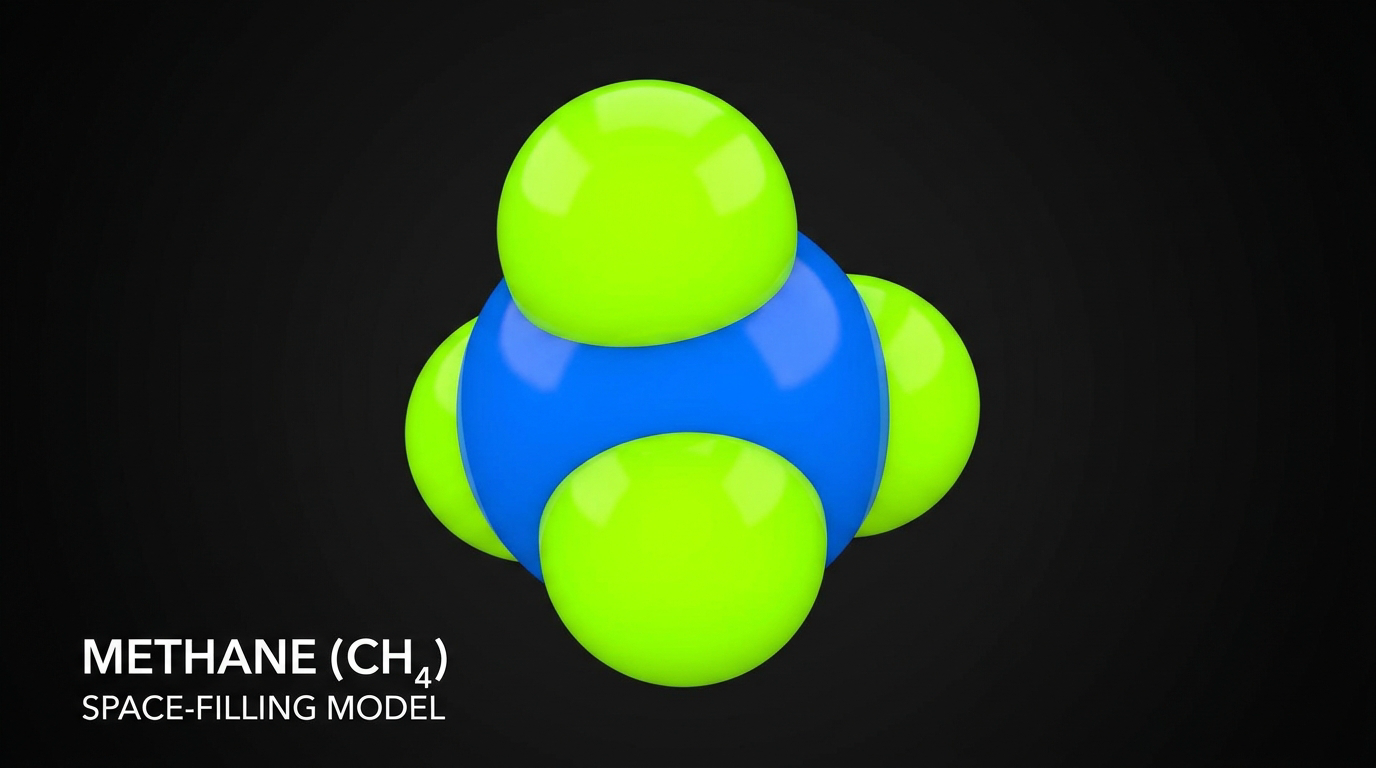
\includegraphics[width=\linewidth]{assets/figures/space_filling.png}
			{\footnotesize\color{softgray} Space-filling}
		\end{center}
		\column{0.24\textwidth}
		\begin{center}
			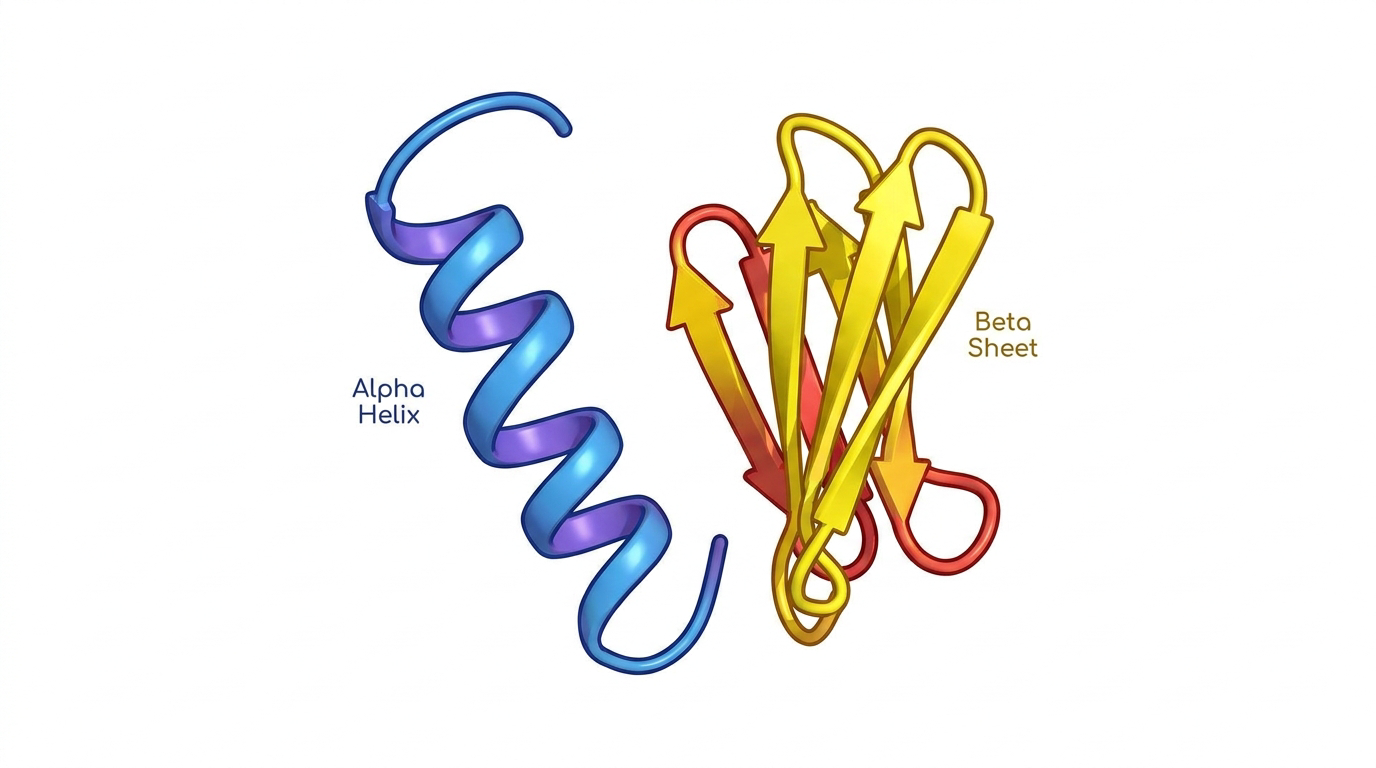
\includegraphics[width=\linewidth]{assets/figures/protein_cartoon.png}
			{\footnotesize\color{softgray} Cartoon}
		\end{center}
	\end{columns}
\end{frame}

\subsection{Objectives \& Applications}
\begin{frame}{Simulation Objectives --- What Are We After?}
	\begin{columns}[T,onlytextwidth]
		\column{0.5\textwidth}
		\begin{pitemize}
			\item \textbf{Structure}: $g(r)$, SASA, clustering
			\item \textbf{Dynamics}: $D$, $\tau$, rates
			\item \textbf{Thermodynamics}: $\Delta G$, $K_d$, phase
			\item \textbf{Mechanism}: pathway, $ PMF$
			\item \textbf{Design}: new molecule / material
		\end{pitemize}
		\column{0.5\textwidth}
		\begin{infobox}[Success = Question + Model + Sampling]
			\footnotesize Bad question + good model = noise\\\small Good question + bad model = \color{neonpink}lie
		\end{infobox}
		\vspace{2mm}
		\begin{tikzpicture}
			\node[draw=accentcyan,fill=accentcyan!15,rounded corners=1mm,inner sep=2mm,text=bgblack] {Drug binding \ensuremath{\rightarrow} Materials \ensuremath{\rightarrow} Energy \ensuremath{\rightarrow} Bio};
		\end{tikzpicture}
	\end{columns}
\end{frame}

\begin{frame}{Applications --- Where It Matters}
	\begin{columns}[T,onlytextwidth]
		\column{0.5\textwidth}
		\begin{pitemize}
			\item Pharma: binding $\Delta G$, \textbf{AlphaFold+MD}
			\item Materials: battery, polymer, catalyst
			\item Energy: CO2 capture, membranes
			\item Life: folding, crowding, rare events
		\end{pitemize}
		\column{0.5\textwidth}
		\memeinclude[width=0.95\linewidth]{assets/memes/intro_meme.png}
	\end{columns}
\end{frame}

\begin{frame}{Interpretation --- Objectives}
	\interpret{
		\textbf{Objectives} · \textbf{structure} / \textbf{dynamics} / \textbf{thermodynamics} · \textbf{mechanism} over movie · \textbf{design} is the test · \textbf{applications} drive approximations
	}
\end{frame}
